%%%%%% Gennemførsel %%%%%%
\chapter{Gennemførsel}

\vspace{-10pt}

Projektet udarbejdes efter RUP modellen. RUP er en arbejdsmodel bestående af de 4 overordnede faser: Inception, Elaboration, Construction og Transition.

Under Inception fasen fastligges projektets problemstilling og krav udarbejdes.
Elaboration er design fase. I denne fasen nedbrydes systemet i mindre blokke, 
og der laves detaljerede beskrivelser af hvilke funktionalitet de forskellige blokke har.
I elaboration udarbejdes desuden beskrivelse af hvordan alle blokke kommunikerer og arbejder sammen.  
I construction fasen konstrueres systemet. I begyndelsen af construction fasen, holdes fokus på de
moduler der udgør systemets grundfunktionalitet. Moduler der skaber grundfunktionalitet kaldes “Need to have”, mens udvidelser kaldes “Nice to have” og sættes som lavere prioritet.
Transistion fasen er den sidste, i denne fase afrundes projektet. Der skrives dokumentation og en rapport der bla. indeholder information om systemet, resultater og en konklusion.


Nedenfor er skitseret en tidsplan, som er sat op efter RUP's 4 faser.
Bemærk at construction fasen er delt i 4 mindre iterations faser.
I den første fase sættes fokus på kommunikation link mellem quadrocopter og webapplikation.
Derefter ændres fokus til GPS, så det bliver muligt for quadrocopter at flyve til en given position.
Senere arbejdes der med at tage, sende og opbevare billeder.
I sidste iteration laves nice to have ting, fx et flot GUI.


%\vspace{-5pt}

\begin{figure}[H]
\centering
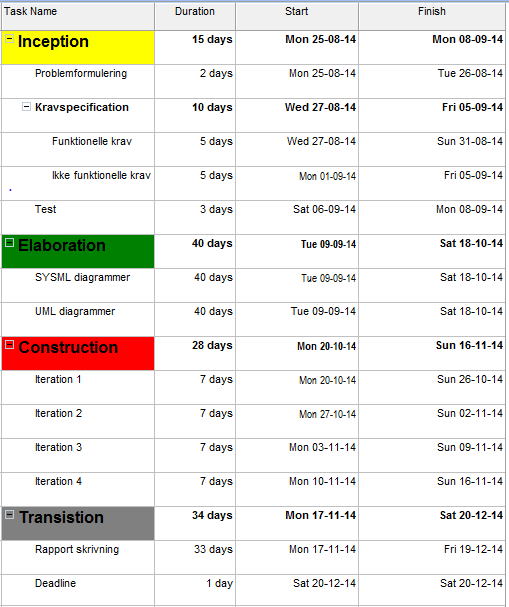
\includegraphics[width=0.5\textwidth]{Billeder/Tidsplan.png}
\caption{Tidsplan}
\label{fig:Tidsplan}
\end{figure}

\newpage


\begin{figure}
\centering
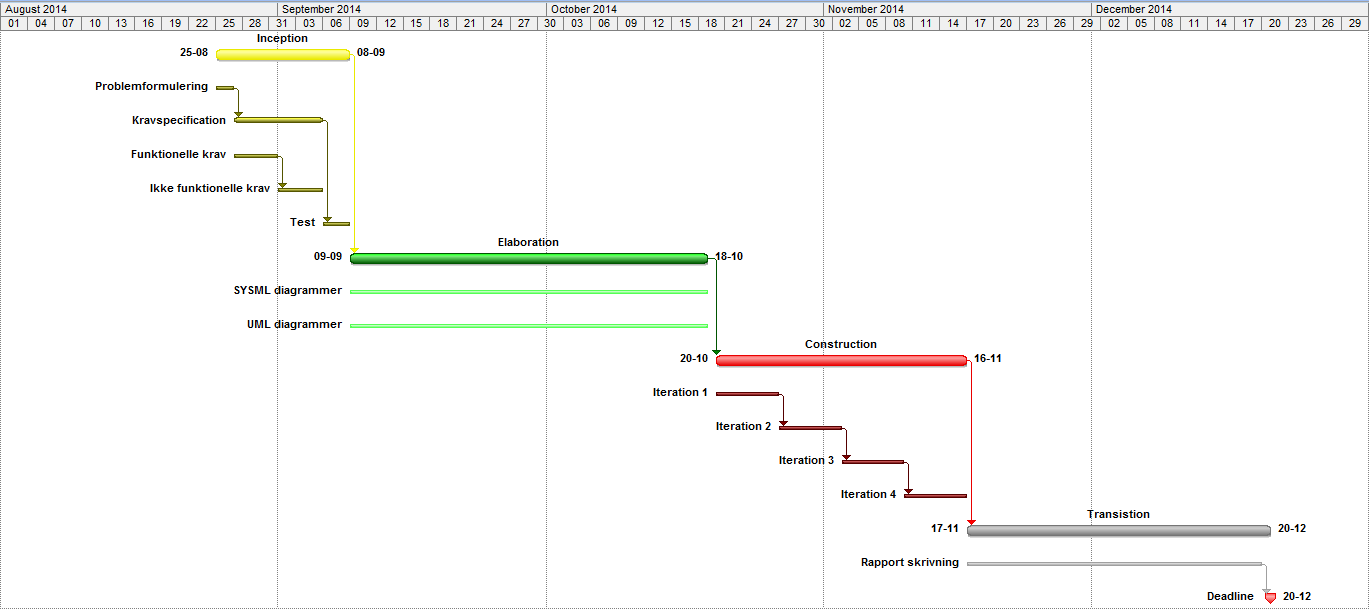
\includegraphics[width=0.7\textwidth]{Billeder/Tidsplan1.png}
\caption{Grafisk tidsplan}
\label{fig:Grafisk_tidsplan}
\end{figure}